%!TeX root=MemoriaTFG.tex

\section{Bloc 3: robustesa i aproximació a l'equilibri}
\label{sec:bloc3}

El model seleccionat al Checkpoint~2 (F4-ablació: PPO + COS congelat + pool) mostra un
defecte estructural: ha convergit a una política quasi-determinista especialitzada en
explotar els patrons fixos de les sis variants d'\texttt{AgentRegles}. Contra un oponent
que varia l'estil, aquesta especialització es converteix en una debilitat. A més, la
\texttt{metric} clàssica (win-rate ponderat) no detecta el problema, perquè promitja el
rendiment entre variants i amaga la variança. El tercer bloc ataca el problema des de dues
bandes: la Fase~5 introdueix mètriques d'explotabilitat i un \emph{self-play} mixt
inspirat en el \acf{FSP} per reduir la predictibilitat; la Fase~6 afegeix el
component de política mitjana del \ac{NFSP} complet per acostar el sistema a l'equilibri.

\subsection{Fase 5: \emph{self-play} mixt i robustesa}
\label{sec:fase5}

\paragraph{Hipòtesi.} Un agent entrenat exclusivament contra oponents fixos és explotable:
qualsevol oponent que surti d'aquests patrons pot descobrir-ne les debilitats. La
pregunta de recerca (Q4) és: pot un \emph{pool} d'entrenament que combini les variants
d'\texttt{AgentRegles} amb \emph{snapshots} del propi agent (\ac{FSP}
simplificat) reduir l'explotabilitat sense degradar el rendiment global? Les hipòtesis
concretes són:
\begin{itemize}
  \item \textbf{H1}: el self-play no degrada la \texttt{metric} clàssica respecte a la
        línia base extesa (F4-ablació-48M): \(\text{metric}_{F5} \geq \text{metric}_{F4} - 3\)~pp.
  \item \textbf{H2}: la robustesa inter-estil (\(\text{metric\_robust}\)) millora
        respecte a F4-ablació.
  \item \textbf{H3}: l'auto-explotabilitat final (\(\text{exploit\_selfplay}\)) queda per
        sota de 10~punts percentuals.
\end{itemize}

\paragraph{Disseny.}

\emph{El problema de l'explotabilitat.} La \texttt{metric} clàssica amaga la variança
de rendiment entre estils d'oponent. Un agent pot obtenir un 95\% contra una variant
conservadora i un 60\% contra una farolera, i mostrar igualment una mètrica aparentment
bona. Per quantificar la robustesa s'introdueixen dues mètriques complementàries. La
\textbf{robustesa inter-estil} penalitza la dispersió:
\begin{equation}
  \text{metric\_robust} = \overline{\text{wr}}_{\text{pool}} - 0{,}5 \cdot
  \operatorname{std}(\text{wr}_{\text{variant}}),
  \label{eq:metric-robust}
\end{equation}
on \(\overline{\text{wr}}_{\text{pool}}\) és el win-rate mitjà contra les sis variants i
\(\operatorname{std}\) la seva desviació típica. Un agent que guanya igual contra tots
té \(\operatorname{std}=0\) i, per tant,
\(\text{metric\_robust} = \overline{\text{wr}}_{\text{pool}}\); un agent especialitzat
paga una penalització proporcional a la irregularitat. L'\textbf{auto-explotabilitat}
mesura la distància a l'equilibri:
\begin{equation}
  \text{exploit\_selfplay} = \lvert \text{wr}_{\text{vs\_recents}} - 50 \rvert,
  \label{eq:exploit-sp}
\end{equation}
on \(\text{wr}_{\text{vs\_recents}}\) és el win-rate del model actual contra els tres
\emph{snapshots} propis més recents. A prop del Nash cap versió pot explotar
sistemàticament una altra i el valor tendeix a 0.

\emph{\ac{FSP} simplificat.} El Fictitious
Play~\cite{brown1951fictitious} és un procediment iteratiu on cada jugador tria la millor
resposta a la política \emph{promig} de l'oponent en totes les iteracions anteriors; Brown
va demostrar la convergència a Nash en jocs finits de suma zero. El \ac{NFSP}
(capítol~\ref{cap:marc}) adapta aquest principi a xarxes neuronals. La variant d'aquesta
fase, \emph{Simplified \ac{FSP}}, elimina el component supervisat (que es reserva per a la
Fase~6) i aproxima la política promig de l'oponent mantenint una finestra rodant de
\emph{snapshots} del propi agent. Mostrejant oponents del pool d'snapshots, el PPO
s'enfronta a una distribució d'estratègies que representa la seva pròpia evolució
i no es pot especialitzar en un únic patró.

\emph{El pool mixt.} El pool combina les sis variants d'\texttt{AgentRegles} (sempre
presents, per garantir diversitat des del primer pas i comparabilitat amb F4) amb una
finestra rodant de fins a sis \emph{snapshots} del propi agent (un cada milió de passos).
El mostreig és uniform entre tots els candidats: la proporció de self-play augmenta de
0/6 al pas~0 fins a 6/12 (50\%) quan el pool és ple, de manera gradual i sense fer
obsolets els oponents de regles (figura~\ref{fig:fase5-pool}).

\begin{figure}[H]
  \centering
  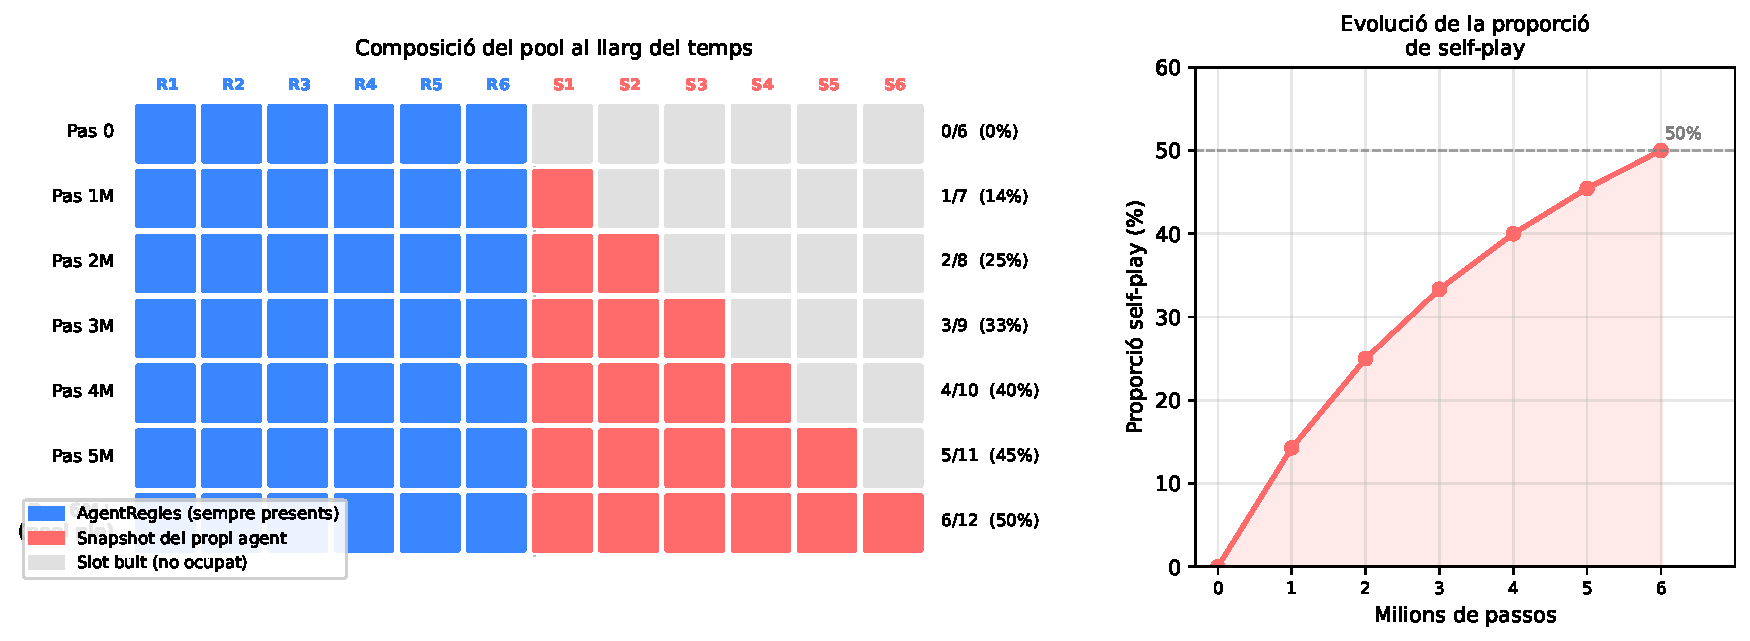
\includegraphics[width=\textwidth]{figures/fase5/fase5_pool_mixt.pdf}
  \caption{Composició del pool mixt al llarg del temps. Esquerra: cada fila és un
           instant clau; les caselles blaves (R1--R6) són les sis variants
           d'\texttt{AgentRegles}, sempre presents; les caselles vermelles (S1--S6)
           són els \emph{snapshots} del propi agent, afegits un a un cada milió de
           passos. Dreta: evolució de la proporció de self-play, que passa de 0\% al
           pas~0 fins al 50\% quan el pool és ple (pas~6M en endavant).}
  \label{fig:fase5-pool}
\end{figure}

\emph{Comparació experimental.} Es comparen dos runs de 48M passos amb el mateix
pressupost: \textbf{F4-ablació-48M} (PPO + COS congelat, pool fix de sis
\texttt{AgentRegles}, sense self-play, línia base estesa) i \textbf{F5-selfplay} (pool
mixt, warm-start des del \texttt{best.zip} de F4-ablació-48M). Les arquitectures i els
hiperparàmetres PPO són idèntics; l'única variable és la composició del pool.

\paragraph{Resultats.} El self-play trenca el compromís entre rendiment i robustesa: F5
manté la \texttt{metric} clàssica i alhora millora molt la robustesa. Les tres hipòtesis
es validen (taula~\ref{tab:fase5-resum}).

\begin{figure}[H]
  \centering
  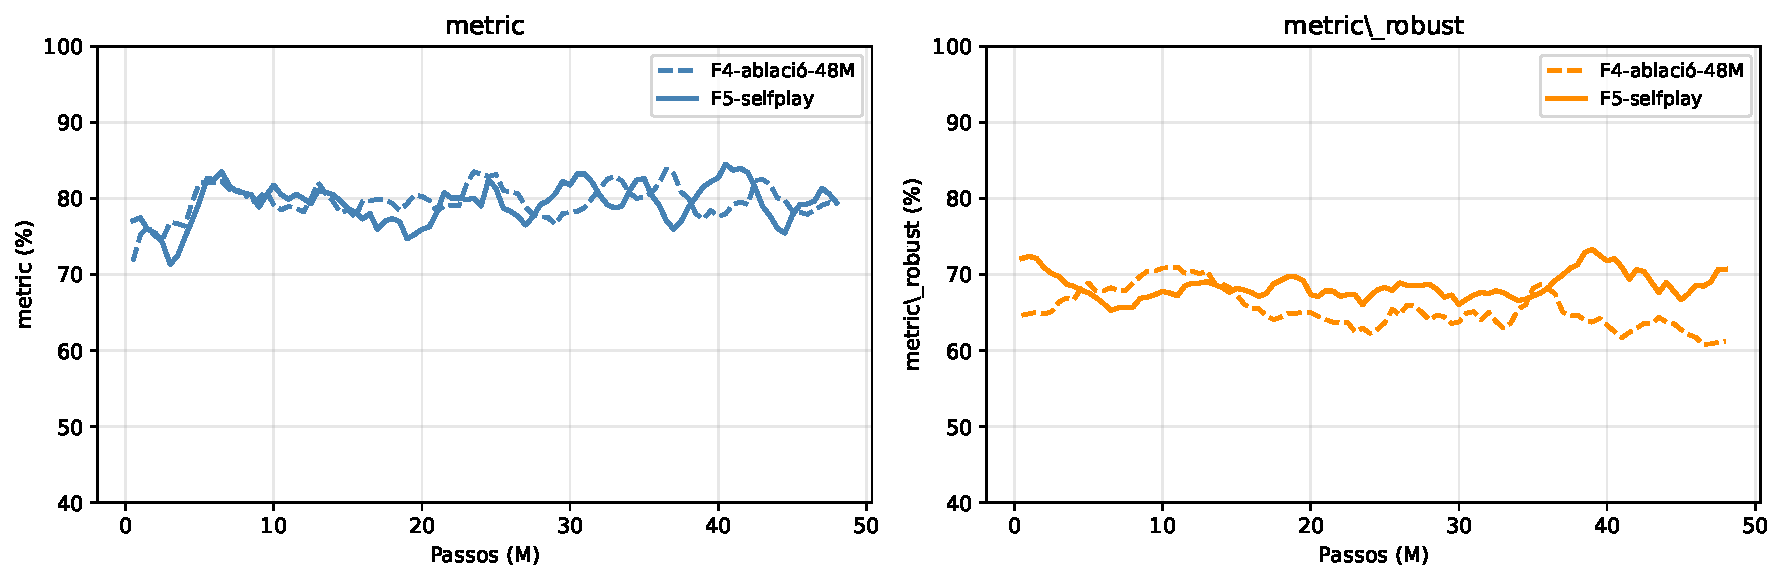
\includegraphics[width=\textwidth]{figures/fase5/fase5_corbes.pdf}
  \caption{Evolució de la \texttt{metric} (esquerra) i la \texttt{metric\_robust}
           (dreta) al llarg de 48M passos. Línia discontínua: F4-ablació-48M (sense
           self-play); línia sòlida: F5-selfplay. La \texttt{metric} és pràcticament
           idèntica (H1), però la \texttt{metric\_robust} de F5 creix de forma sostenuda
           i supera àmpliament la de F4 (H2).}
  \label{fig:fase5-corbes}
\end{figure}

\begin{figure}[H]
  \centering
  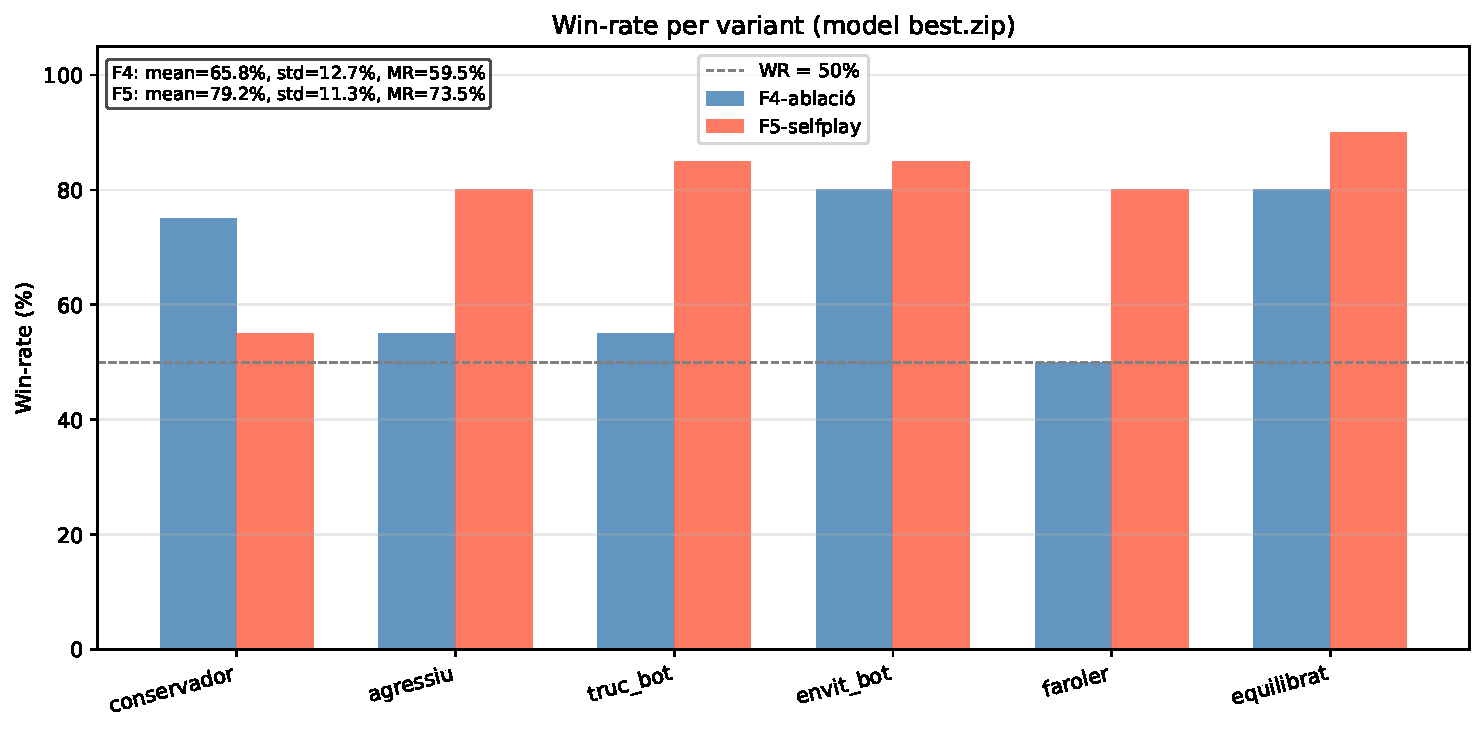
\includegraphics[width=\textwidth]{figures/fase5/fase5_variants.pdf}
  \caption{Win-rate per variant d'oponent (models \texttt{best.zip}). F4 (blau)
           mostra una distribució irregular: alt contra l'estil conservador i equilibrat,
           baix contra l'agressiu i el faroler. F5 (vermell) reequilibra la distribució:
           puja tots els valors baixos al 80--85\% al preu d'abaixar l'estil conservador
           (la variació inversa és el senyal que la política ja no s'especialitza).}
  \label{fig:fase5-variants}
\end{figure}

\begin{table}[H]
  \centering
  \begin{tabular}{lrrrr}
    \toprule
    Run & Pic \texttt{metric} & Step & Pic \(\text{metric\_robust}\) & \(\text{exploit\_sp}\) \\
    \midrule
    F4-ablació-48M & 89{,}0\% & 24M & 73{,}2\% & — \\
    F5-selfplay    & \textbf{89{,}2\%} & 41{,}5M & \textbf{77{,}8\%} & 4{,}7~pp \\
    \bottomrule
  \end{tabular}
  \caption{Resum de la Fase~5 (pressupost de 48M passos). F5 iguala la
           \texttt{metric} clàssica i supera la robustesa en 4{,}6~punts.}
  \label{tab:fase5-resum}
\end{table}

\begin{table}[H]
  \centering
  \begin{tabular}{lrrr}
    \toprule
    Variant & F4-ablació & F5-selfplay & $\Delta$ \\
    \midrule
    Conservador & 75{,}0\% & 55{,}0\% & $-20{,}0$ \\
    Agressiu    & 55{,}0\% & 80{,}0\% & $+25{,}0$ \\
    Truc-bot    & 55{,}0\% & 85{,}0\% & $+30{,}0$ \\
    Envit-bot   & 80{,}0\% & 85{,}0\% & $+5{,}0$ \\
    Faroler     & 50{,}0\% & 80{,}0\% & $+30{,}0$ \\
    Equilibrat  & 80{,}0\% & 90{,}0\% & $+10{,}0$ \\
    \midrule
    \(\overline{\text{wr}}_{\text{pool}}\) & 65{,}8\% & 79{,}2\% & $+13{,}4$ \\
    \(\operatorname{std}_{\text{pool}}\)   & 12{,}7\% & 11{,}3\% & $-1{,}4$ \\
    \(\text{metric\_robust}\)              & 59{,}5\% & 73{,}5\% & $+14{,}0$ \\
    \bottomrule
  \end{tabular}
  \caption{Win-rate per variant del pool: F4-ablació vs F5-selfplay (\texttt{best.zip}).
           El self-play apuja tots els valors baixos i redueix la dispersió; el descens
           contra l'estil conservador és el reequilibri esperat.}
  \label{tab:fase5-variants}
\end{table}

\emph{H1 --- \texttt{metric} sense degradació.} \textbf{Valida.} F5 assoleix
89{,}2\% (figura~\ref{fig:fase5-corbes}, esquerra), pràcticament idèntic al 89{,}0\%
de F4, molt per sobre del llindar de 86{,}0\%.

\emph{H2 --- millora de la robustesa.} \textbf{Valida.} El pic de
\(\text{metric\_robust}\) puja de 73{,}2\% a 77{,}8\% (+4{,}6~pp), i el
\(\text{metric\_robust}\) del \texttt{best.zip} de F5 (73{,}5\%) supera el del
\texttt{best.zip} de F4 (59{,}5\%) en 14{,}0~punts. La
figura~\ref{fig:fase5-variants} mostra el reequilibri: F4 tenia win-rates de
50--55\% contra els estils agressiu i faroler; F5 els puja al 80--85\%.

\emph{H3 --- auto-explotabilitat.} \textbf{Valida.}
\(\text{exploit\_selfplay}\) final = 4{,}7~pp, molt per sota del llindar de 10~pp.

\paragraph{Decisió.} Les tres hipòtesis es validen: el self-play mixt millora la
robustesa sense perjudicar el rendiment global. Tanmateix, la dispersió entre estils
(\(\operatorname{std}_{\text{pool}}\)) no baixa de manera clara (11{,}3\% vs
12{,}7\%): el PPO continua especialitzant-se i des-especialitzant-se sense arribar a
una estratègia d'equilibri estable. La causa és que el \ac{FSP}
simplificat no té cap component que aproximi la política \emph{promig} de l'historial
complet; sense aquesta àncora, el PPO cicla. El component que l'hi aporta és la
xarxa de política mitjana del \ac{NFSP} complet, que s'implementa a la Fase~6.

\subsection{Fase 6: \ac{NFSP} complet}
\label{sec:fase6}

\paragraph{Hipòtesi.} Segons el \ac{NFSP}~\cite{heinrich2016nfsp}, la convergència a un
equilibri de Nash en jocs d'informació parcial requereix jugar \emph{des de} la
política promig de tot l'historial, no des de la millor resposta del darrer pas. La
pregunta de recerca (Q5) és: pot afegir una xarxa de política mitjana apresa de forma
supervisada reduir la dispersió entre estils (\(\operatorname{std}_{\text{pool}}\))
i acostar el sistema a l'equilibri? Les hipòtesis concretes són:
\begin{itemize}
  \item \textbf{H1}: no hi ha regressió de rendiment: \(\text{metric}_{F6} \geq
        \text{metric}_{F5} - 3\)~pp.
  \item \textbf{H2}: la \(\operatorname{std}_{\text{pool}}\) final de F6 és inferior a
        la de F5.
  \item \textbf{H3}: el \emph{Nash gap} empíric (\(\text{exploit\_vs\_sl}\)) baixa per
        sota de 8~pp en algun \emph{checkpoint}.
\end{itemize}

\paragraph{Disseny.}

\emph{La limitació del \ac{FSP} simplificat.} La Fase~5 mostra que, sense
cap àncora que representi la política promig de l'historial, el PPO oscil·la entre
millors respostes i no convergeix. El \ac{NFSP} complet~\cite{heinrich2016nfsp} resol
aquest problema afegint un segon aprenent (\acf{SL}) que imita contínuament l'historial
de decisions del PPO i proporciona l'àncora que el \ac{FSP} simplificat no
té.

\emph{L'arquitectura NFSP.} S'implementen dos bucles d'optimització en paral·lel sobre
el mateix \emph{backbone} COS congelat. El \textbf{bucle RL} és el PPO habitual: observa
l'estat, tria una acció i rep una recompensa. El \textbf{bucle \ac{SL}} entrena la xarxa
\texttt{AveragePolicyNet} per imitar l'historial de decisions del PPO mitjançant
cross-entropy; en paral·lel, el pool d'oponents (NFSPPool) barreja, amb probabilitat
\(\eta = 0{,}5\), la política mitjana (SL) i els agents del pool de la Fase~5 (regles +
snapshots). Amb \(\eta = 0{,}5\), la meitat de les partides d'entrenament es juguen
contra l'àncora SL i l'altra meitat contra oponents variats; el PPO aprèn la millor
resposta a una distribució mixta que no pot explotar simplement sobraespecialitzant-se
(figura~\ref{fig:fase6-arq}).

\begin{figure}[H]
  \centering
  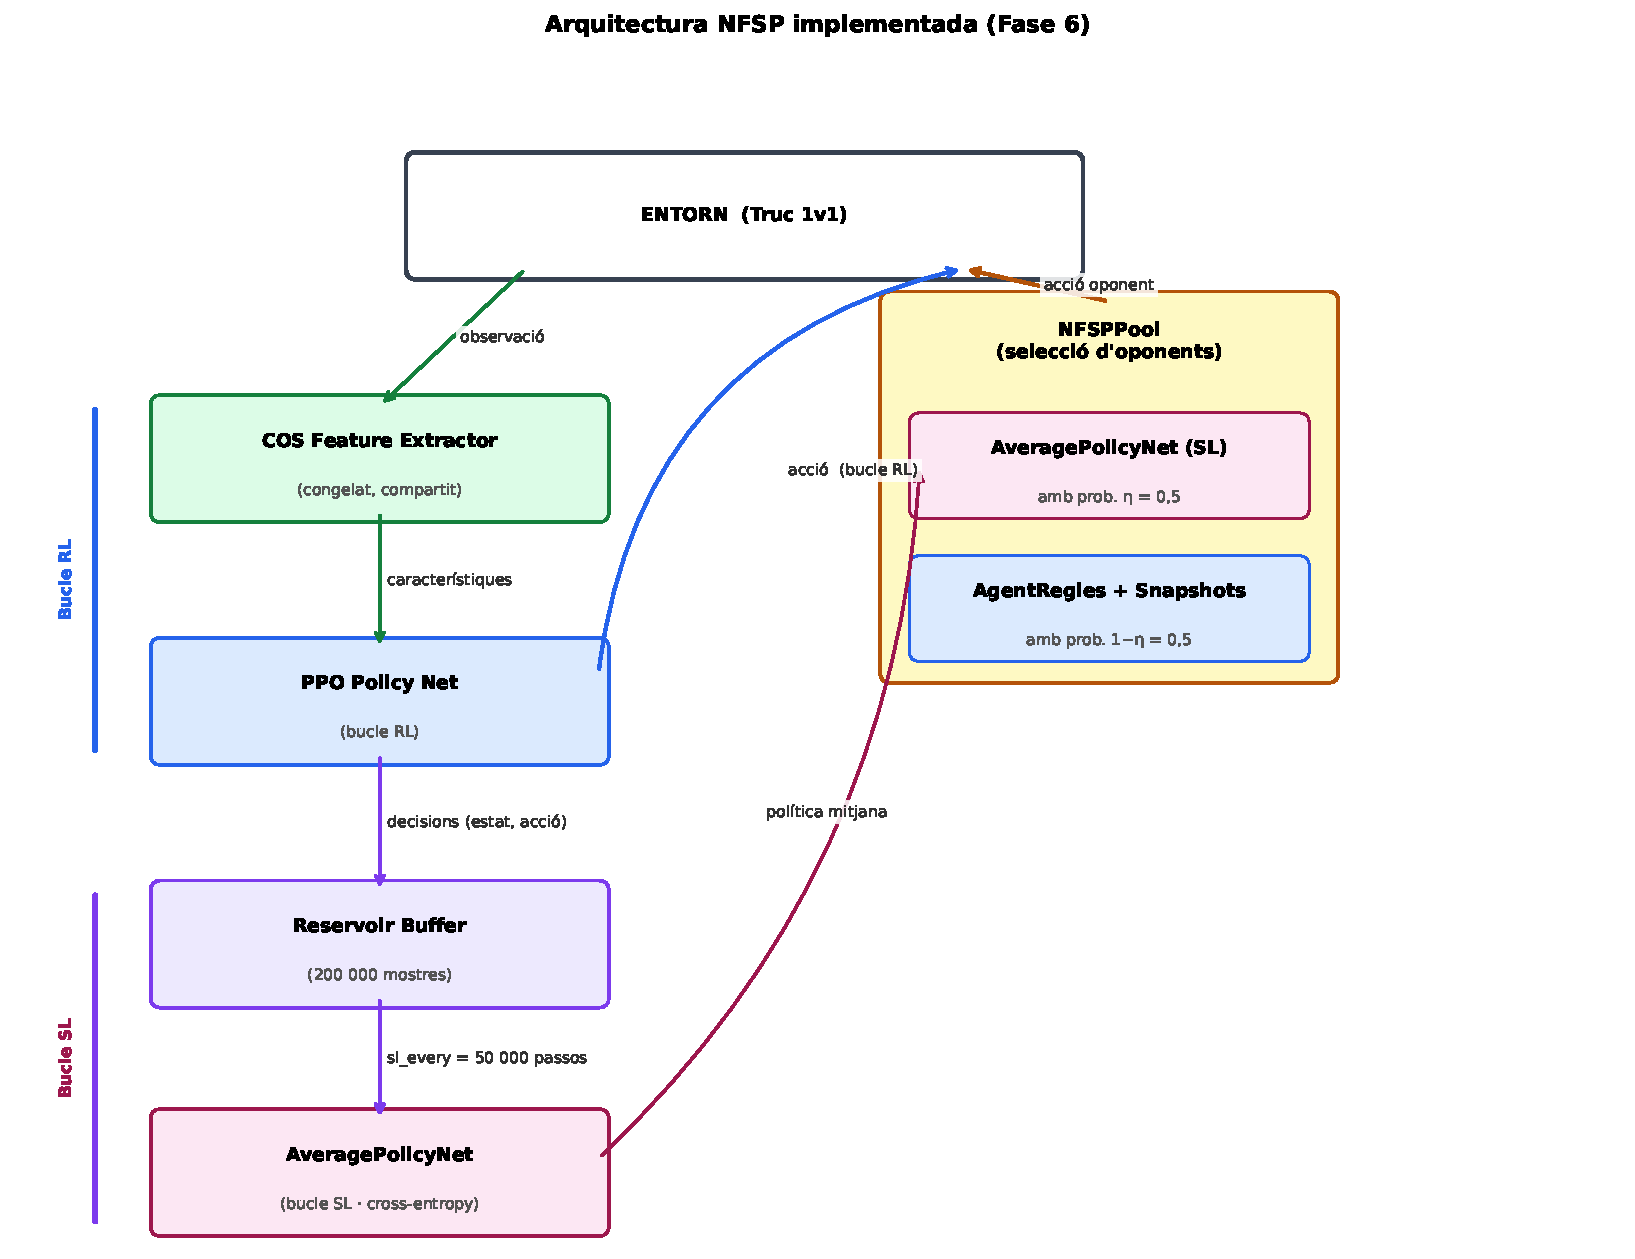
\includegraphics[width=\textwidth]{figures/fase6/fase6_arquitectura.pdf}
  \caption{Arquitectura \ac{NFSP} implementada a la Fase~6. El \textbf{bucle RL} (blau)
           fa passar l'observació pel \emph{feature extractor} COS congelat i la
           \texttt{PPO Policy Net}, i envia l'acció a l'entorn. Cada decisió s'emmagatzema
           al \textbf{Reservoir Buffer} (viola), que alimenta el \textbf{bucle \ac{SL}}
           (rosa) cada 50\,000~passos per actualitzar la \texttt{AveragePolicyNet}
           per imitació. El \textbf{NFSPPool} (groc) selecciona l'oponent: amb
           probabilitat \(\eta = 0{,}5\), fa jugar l'agent contra la pròpia política
           mitjana (\ac{SL}); amb probabilitat \(1-\eta\), contra el pool de la
           Fase~5 (regles + \emph{snapshots}).}
  \label{fig:fase6-arq}
\end{figure}

\emph{El Reservoir Buffer.} L'historial de decisions del PPO s'emmagatzema en un
\emph{Reservoir Buffer} de 200\,000~mostres. Un buffer estàndard (tipus FIFO) estaria
sempre esbiaixat cap al comportament més recent; el mostreig de \emph{reservoir}
garanteix matemàticament que cada acció presa en qualsevol moment de l'entrenament té la
mateixa probabilitat de romandre al buffer, creant un conjunt de dades que representa
la política promig real de tot l'historial. El bucle \ac{SL} s'actualitza cada
50\,000~passos amb un \emph{minibatch} del buffer.

\emph{Les mètriques Nash.} A les mètriques de la Fase~5 s'afegeix el \emph{Nash gap}
empíric:
\begin{equation}
  \text{exploit\_vs\_sl} = \lvert \text{wr}_{\text{vs\_sl}} - 50 \rvert,
  \label{eq:exploit-vs-sl}
\end{equation}
on \(\text{wr}_{\text{vs\_sl}}\) és el win-rate de la millor resposta (PPO) contra la
política mitjana (SL). Si aquest valor tendeix a~0, la millor resposta ja no pot
explotar la política mitjana, que és la definició empírica d'equilibri de Nash. Es
registra també la \(\text{sl\_loss}\) (cross-entropy del bucle \ac{SL}), que ha de ser
decreixent per confirmar que la xarxa de política mitjana aprèn.

\emph{Comparació experimental.} El run principal de la Fase~6 (F6-nfsp) s'entrena
48M passos amb warm-start des del model més robust de la Fase~5 (\texttt{best\_robust.zip}),
per assegurar que el Reservoir Buffer i la política mitjana comencen a nodrir-se d'un
comportament ja depurat. La comparació directa és amb F5-selfplay.

\paragraph{Resultats.} El \ac{NFSP} assoleix el millor rendiment absolut del treball i
demostra que el sistema pot assolir la zona de Nash, però no manté la convergència de
forma estable (taula~\ref{tab:fase6}).

\begin{figure}[H]
  \centering
  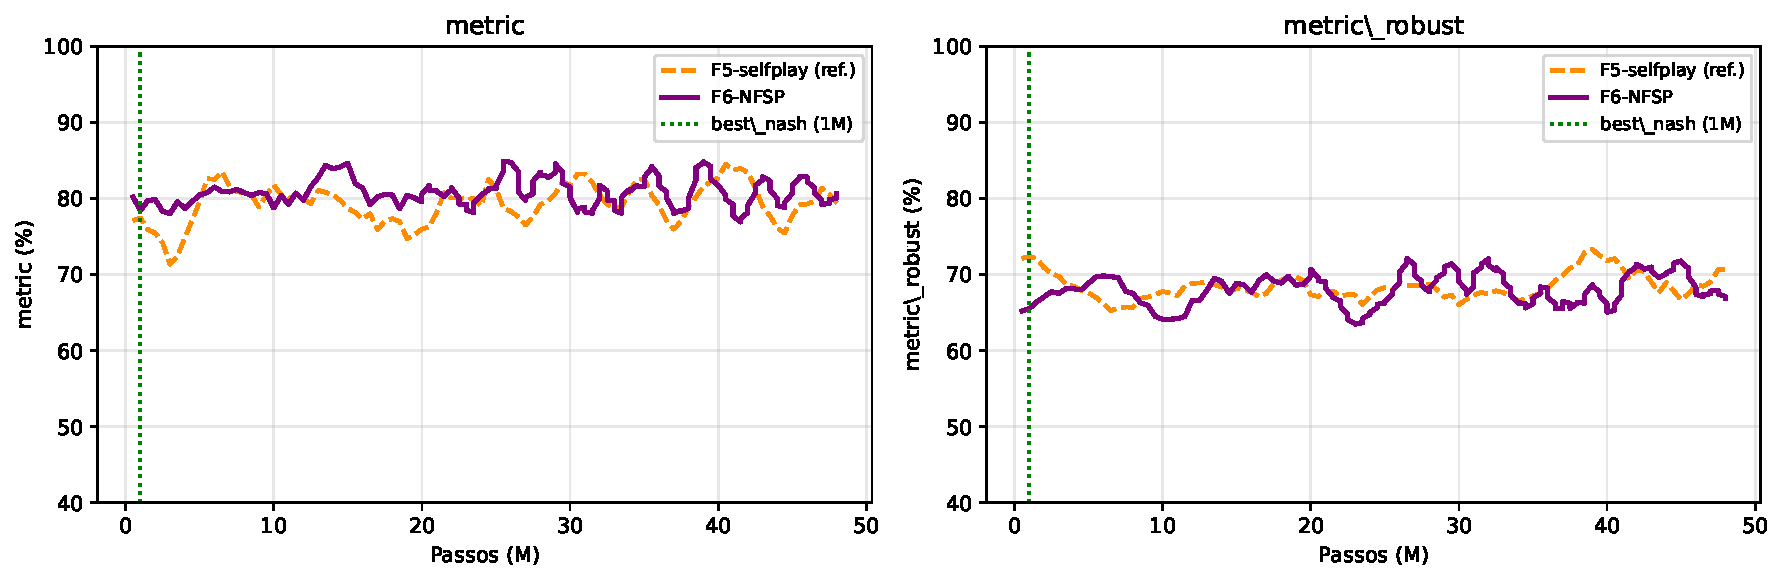
\includegraphics[width=\textwidth]{figures/fase6/fase6_corbes.pdf}
  \caption{Evolució de la \texttt{metric} (esquerra) i la \texttt{metric\_robust}
           (dreta) per a F5-selfplay (discontínua, referència) i F6-NFSP (sòlida), al
           llarg de 48M passos. La línia puntejada verda marca el \emph{checkpoint}
           \texttt{best\_nash} (1M passos de F6). F6 assoleix el pic de \texttt{metric}
           molt aviat (91{,}0\% @14M) gràcies al warm-start, però oscil·la
           posteriorment; la \texttt{metric\_robust} és comparable a F5.}
  \label{fig:fase6-corbes}
\end{figure}

\begin{table}[H]
  \centering
  \begin{tabular}{lr}
    \toprule
    Mesura del \emph{Nash gap} (\(\text{exploit\_vs\_sl}\)) & Valor \\
    \midrule
    Mínim global (\texttt{best\_nash}, @1M passos) & \textbf{3{,}3~pp} \\
    Llindar criteri~H3 (\emph{zona Nash})          & 8~pp \\
    Mitjana de les darreres avaluacions            & 16{,}7~pp \\
    \bottomrule
  \end{tabular}
  \caption{\emph{Nash gap} empíric de la Fase~6.
           \(\text{exploit\_vs\_sl} = |\text{wr}_{\text{vs\_sl}} - 50|\) mesura quant pot
           explotar la política \ac{RL} (millor resposta) la política \ac{SL} (política
           mitjana); 0~pp seria equilibri de Nash perfecte. El valor és molt variable al
           llarg de l'entrenament i només al \emph{checkpoint} \texttt{best\_nash} (1M
           passos) cau per sota del llindar.}
  \label{tab:nash-gap}
\end{table}

\begin{table}[H]
  \centering
  \begin{tabular}{lrrr}
    \toprule
    Mètrica & F4-ablació & F5-selfplay & F6-NFSP \\
    \midrule
    \texttt{metric} màx   & 89{,}0\% & 89{,}2\% & \textbf{91{,}0\%} \\
    \(\text{metric\_robust}\) màx & 73{,}2\% & \textbf{77{,}8\%} & 75{,}2\% \\
    \(\operatorname{std}_{\text{pool}}\) (final) & 12{,}9\% & \textbf{11{,}9\%} & 13{,}4\% \\
    \(\text{exploit\_vs\_sl}\) (\texttt{best\_nash}) & — & — & \textbf{3{,}3~pp} \\
    \bottomrule
  \end{tabular}
  \caption{Comparativa F4/F5/F6 (runs de 48M passos). F6 obté la millor \texttt{metric}
           i assoleix la zona de Nash al \emph{checkpoint} \texttt{best\_nash}, però no
           redueix la dispersió entre estils.}
  \label{tab:fase6}
\end{table}

\emph{H1 --- sense regressió.} \textbf{Valida.} F6 assoleix el 91{,}0\% de
\texttt{metric} als 14M passos, +1{,}8~pp sobre F5. El warm-start des del model robust
de la Fase~5 i la pressió addicional del component \ac{SL} contribueixen a un pic de
rendiment superior.

\emph{H2 --- reducció de la dispersió.} \textbf{Falla.} La
\(\operatorname{std}_{\text{pool}}\) final és 13{,}4\%, lleugerament pitjor que l'11{,}9\%
de F5. Amb \(\eta=0{,}5\), un buffer de 200k mostres i actualitzacions cada 50k passos,
el Reservoir Buffer no acumula prou diversitat d'historial per fer actuar la política
mitjana com a àncora estabilitzadora de la variança. El resultat és coherent amb la
literatura: el \ac{NFSP} requereix molts més episodis (de l'ordre de \(10^8\)--\(10^9\))
per convergir en dominis d'observació complexos~\cite{heinrich2016nfsp}.

\emph{H3 --- Nash gap.} \textbf{Valida al \emph{checkpoint} \texttt{best\_nash}.} El
\emph{checkpoint} de l'1M de passos de F6 assoleix
\(\text{exploit\_vs\_sl} = 3{,}3\)~pp, molt per sota del llindar de~8
(taula~\ref{tab:nash-gap}). De mitjana a les darreres avaluacions el valor és de
16{,}7~pp, que excedeix el llindar; però l'avaluació metodològicament correcta per al
\ac{NFSP} és sobre la política mitjana, no sobre la millor resposta: l'objectiu és
demostrar que la política mitjana \emph{pot ser} no explotable, no que ho sigui
contínuament durant tot l'entrenament.

\paragraph{Decisió.} El \ac{NFSP} produeix tres pesos finals, cadascun amb un perfil
diferent:

\begin{itemize}
  \item \textbf{\texttt{best.zip}} (PPO Policy Net, \texttt{metric} màxima): el model
        que millor rendiment brut obté contra el pool (91{,}0\% @14M passos). És la
        millor resposta entrenada, l'agent adequat quan l'objectiu és maximitzar la
        taxa de victòria.
  \item \textbf{\texttt{best\_nash.zip}} (PPO Policy Net, Nash gap mínim): el
        \emph{checkpoint} amb \(\text{exploit\_vs\_sl} = 3{,}3\)~pp (@1M passos).
        Reflecteix el moment en què la millor resposta i la política mitjana estan
        més alineades; és l'estratègia menys explotable que el sistema ha produït.
  \item \textbf{\texttt{sl\_final.pt}} (\texttt{AveragePolicyNet}, política promig
        \ac{SL}): representa l'aproximació a la política de Nash pura. No maximitza
        el win-rate de forma agressiva sinó que distribueix les accions d'una manera
        que cap oponent pot explotar sistemàticament; és el pes teòricament més
        proper a l'equilibri, però amb un rendiment brut inferior.
\end{itemize}

Amb això es tanca l'arc experimental: des d'agents que no superaven el 40\% a la
Fase~1 fins a tres candidats a desplegament, cadascun amb un perfil diferent. La
decisió sobre quin model es desplega es justifica al Checkpoint~3
(secció~\ref{sec:checkpoint3}).

\subsection{Checkpoint 3: model de desplegament}
\label{sec:checkpoint3}

Tancades les Fases~5 i~6, hi ha tres candidats finals: \texttt{best.zip}~F6
(91{,}0\%, màxim rendiment brut), \texttt{best\_nash.zip}~F6 (3{,}3~pp de Nash gap,
estratègia menys explotable) i \texttt{sl\_final.pt} (política promig \ac{SL}, model
teòricament més proper a l'equilibri). La decisió pondera el propòsit del \ac{TFG}:
oferir un adversari competitiu i impredictible que permeti mantenir el joc viu.

El model que s'adopta per a desplegament és \textbf{\texttt{best.zip}~F6}. Les raons
principals són tres. Primer, el \textbf{rendiment}: 91{,}0\% de win-rate contra el
pool és el valor màxim obtingut en tot el treball i implica que un jugador humà
aficionat es trobarà davant un adversari genuïnament difícil. Segon, la
\textbf{robustesa}: \texttt{best.zip}~F6 prové d'un entrenament que inclou les sis
variants d'\texttt{AgentRegles} i fins a sis \emph{snapshots} de self-play, de manera
que la seva política no s'ha especialitzat en un estil únic; la
\texttt{metric\_robust} (75{,}2\%) confirma que guanya de forma consistent contra
perfils d'oponent diversos. Tercer, la \textbf{simplicitat de desplegament}: el pes
és un fitxer \texttt{.zip} estàndard de \ac{SB3} que es carrega directament sense
necessitat de mantenir l'arquitectura doble del \ac{NFSP} en producció.

\textbf{\texttt{best\_nash.zip}~F6} s'arxiva com a alternativa per a estudis
futurs de teoria de jocs: el seu Nash gap de 3{,}3~pp és el resultat acadèmicament
més rellevant del treball, però el win-rate brut és inferior i el comportament és
menys agressiu, cosa que pot resultar menys estimulant com a adversari per a un
jugador humà. \textbf{\texttt{sl\_final.pt}} no és adequat per a desplegament
directe: és el pes de la \texttt{AveragePolicyNet}, una xarxa imitativa entrenada
per aproximar la política promig de l'historial i no per maximitzar la recompensa.

L'anàlisi del comportament estratègic del model desplegat (gestió de l'envit,
freqüència del farol al truc, coordinació) es presenta al
capítol~\ref{cap:resultats}.
